\subsection{Design of the solution}
This section describes the design of the overall Lapsus solution, with a focus on the system’s structure. The design is based on the knowledge and insights obtained through analysis and the state of art section and translates these into a technical solution.

The section introduces the core system components and their relationships and provides the foundation for the subsequent diagrams that illustrate system interactions and architecture. The purpose is to present a clear and structured overview of how the system is constructed.

\subsubsection{Use case diagram}
The use case diagram (see \autoref{fig:use-case-diagram}) highlights the use cases in the system boundary. Here, it is seen that the user can log in through the backend. The user can also add relatives to the database. Furthermore, the user can connect to the wristband through Bluetooth between the wristband and a phone. The user can also cancel the alarm and press the emergency button, which goes through the database and backend. In the system boundary, the relatives can log in and view the \gls{gps} location of the user in real time, both of which use the backend.

\begin{figure} [H]
    \centering
    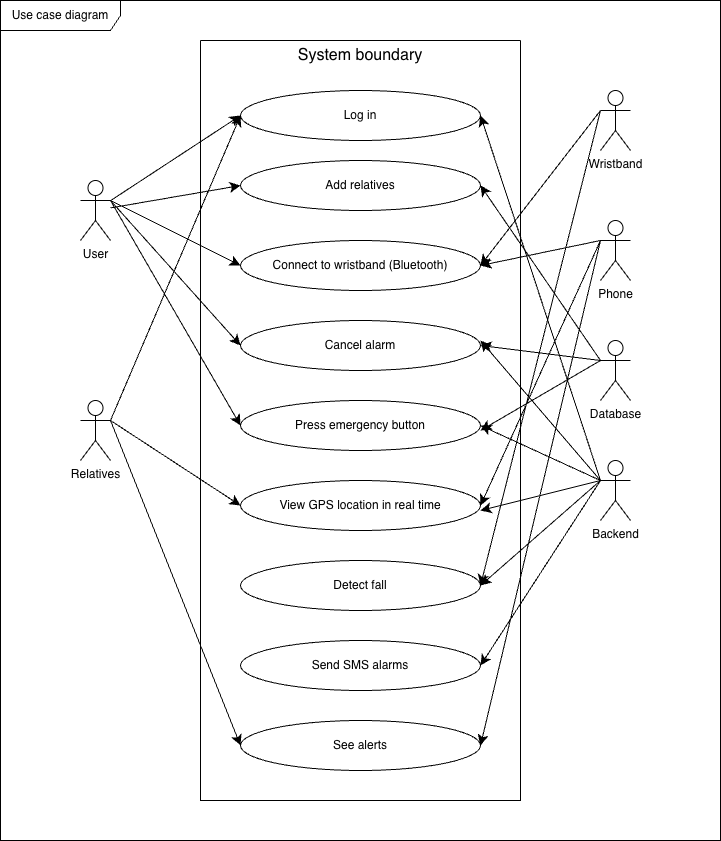
\includegraphics[width=1\linewidth]{report/images/Use case diagram P3.drawio.png}
    \caption{Use case diagram}
    \label{fig:use-case-diagram}
\end{figure}

\subsubsection{Context diagram}
The defined requirements, together with insights from the state of art analysis, form the foundation for the overall system structure of Lapsus. Based on this knowledge, the context diagram was developed to provide a high-level representation of the system and its interaction with external entities. The diagram reflects key design decisions derived from the requirements, including the central role of the mobile application, the exclusion of an internal alarm center, and the reliance on relatives as the primary responders.

The context diagram in \autoref{fig:contextdiagram} gives an overview of the application as a system. Here it is seen that there are four external entities: wristband, user, Firebase and relatives. 
The first dataflow \textit{detect fall} goes from \textit{wristband} to the application. Then, from the user, the data \textit{add relatives} and \textit{cancel alert} flows to the application. From the application, the dataflows \textit{fall detection alert} and \textit{location data} are sent to the relatives. Lastly, the application sends the \textit{add users and relatives}, \textit{location data} and \textit{login request} data to Firebase, where Firebase can send the \textit{list of relatives}, \textit{location history} and \textit{login token (\gls{jwt})} data to the application. 

\begin{figure}[H]
    \centering
    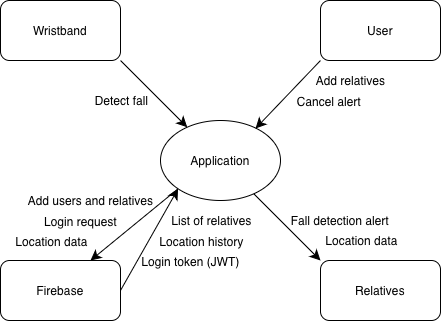
\includegraphics[width=0.75\linewidth]{report//images/Context.drawio.png}
    \caption{Context diagram for the system}
    \label{fig:contextdiagram}
\end{figure}





